\newpage

\chapter{Architektura elektronového děla}
Nejdříve se zaměříme na možné praktické zdroje volných elektronů. Pro potřeby elektronového děla se využívá fotoelektrického jevu -- fotoemise, poté tzv. studené emise elektronů z látky indukované silným elektrickým pole a nejčastěji využívaná termoemise elektronů. Právě termoemise, jako zvolená metoda pro generování volných elektronů, bude důkladněji rozebrána. Dále si představíme námi použitá elektronová děla: vlastní soustavu využívající termoemise z wolframového vlákna se čtyřmi elektrodami a finální setup průmyslového elektronové děla s přidanou soustavou čtyřech elektrod.
\section{Zdroje volných elektronů}
Obecně je nutné dodat elektronům v látce, většinou kovu, dostatečnou energii k překonání vazebných sil s atomy látky, čímž se uvolní do prostoru (uvažujme vakuum). Dochází i k tunelovému jevu, jako je tomu u studené emise. Uvolněné elektrony mohou být následně urychleny elektrostatickým polem.
\subsection{Fotoemise} Tato emise elektronů z látky je způsobena fotoelektrickým jevem, tj. interakcí vázaných elektronů v atomech s externími přilétajícími fotony. Využívá se záporně nabité katody, která je ozařována z vnějšího zdroje fotony o dostatečné frekvenci $f$, resp. energii $hf$ k uvolnění vázaných elektronů v látce. Uvolněné elektrony mají poté ze známého vztahu maximální kinetickou energii rovnu $E_{kin}=hf-W$, kde $W$ je z \textit{work function} -- minimální energie nutná pro uvolnění elektronu z látky. Hovoříme o maximální kinetické energii z důvodu možné realizace Comptonova rozptylu, kdy poté foton nezanechá všechnu svou energii v jedné interakci s elektronem, ale po interakci se šíří dále s nižší frekvencí, resp. energií. Takový zdroj elektronů má poté nediskrétní spektrum, avšak vzhledem k mnohem větším škálám následného urychlení lze tento rozdíl zanedbat. 
\subsection{Studená emise} Název této emise elektronů je dán, kvůli kontrastu s termoemisí. Uvažujme pevnou látku (kov) a přiveďme napěťový spád mezi něj a okolní prostor (vakuum), tak aby emitující materiál byl katodou jako na Obr. \ref{CFEpotent}. Můžeme vidět \textit{field-free potential barrier}, kdy tento potenciál případu bez externího pole zabraňuje elektronům pod Fermiho hladinou opouštět daný materiál a k jeho překonání je potřeba výstupní práce $W$. Přidáme-li však napěťový spád, tím potenciál -- \textit{potential of the applied field}, tak pro uvolnění elektronů z látky je nutné efektivně překonat superponovaný potenciál vyznačený na Obr. \ref{CFEpotent} nepřerušovanou černou čarou. Tato vzniklá potenciálová bariéra může být statisticky elektronem protunelována a daný elektron je poté ve volném prostoru mimo látku a urychlován spádem napětí externího pole. Je nutné dodat, že jak bylo teoreticky předpovězeno, tak úzký hrot látky emituje elektrony snáze, a proto se využívá hrotů jako na Obr. \ref{CFE} vpravo. Celého principu lze například využít u elektronových tunelových mikroskopů, kdy namísto tunelování elektronů do volného prostoru, tunelují do zkoumaného vzorku v určitém počtu úměrném vzdálenosti mezi emitujícím hrotem a povrchem vzorku. 

\begin{figure}[htbp!]
	\centering
	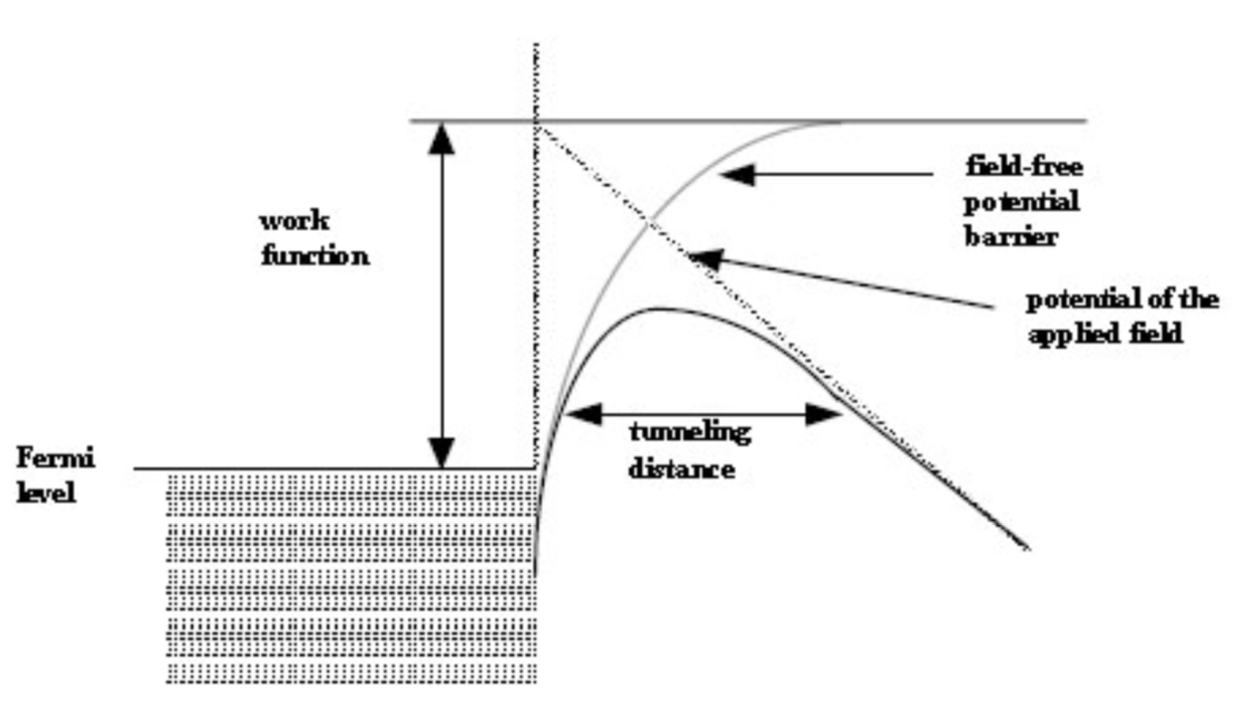
\includegraphics[width = 350 pt]{CFEpotent.png}
	\caption{Průběh potenciálů v blízkosti rozhraní emitující látky a vakua. Převzato z~\cite{coldems}.}
	\label{CFEpotent}
\end{figure}

\begin{figure}[htbp!]
	\centering
	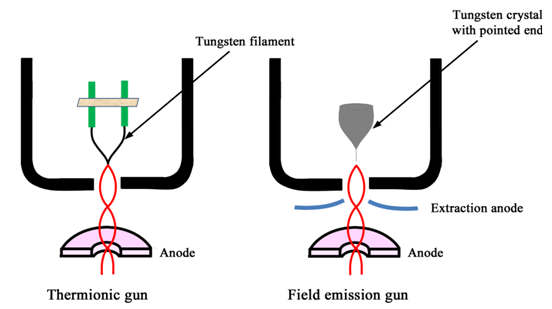
\includegraphics[width = 350 pt]{CFE.png}
	\caption{Schémata možné realizace zdroje elektronů. Vlevo: termoemise elektronů z wolframového vlákna. Vpravo: studená emise elektronů z hrotu krystalu wolframu. Převzato z~\cite{zdrojel}.}
	\label{CFE}
\end{figure}

\subsection{Termoemise}
K uvolnění elektronů lze využít i tepelné energie $kT$, kde $k$ je Boltzmanova konstanta a $T$ je termodynamická teplota. Tato tepelná energie, představující střední kinetickou energii elektronů v látce, může být srovnatelná s výstupní prací elektronů z látky $W$, v tom případě elektrony s dostatečnou energií opouští povrch látky do prostoru. Hustota emisního proudu elektronů $J$ se řídí dle Richardson-Duschmanova zákona:
\begin{equation}
	J=BT^2\exp(-\frac{W}{kT}),
	\label{RDlaw}
\end{equation}
kde $B$ je charakteristická konstanta každého materiálu. 
\begin{figure}[htbp!]
	\centering
	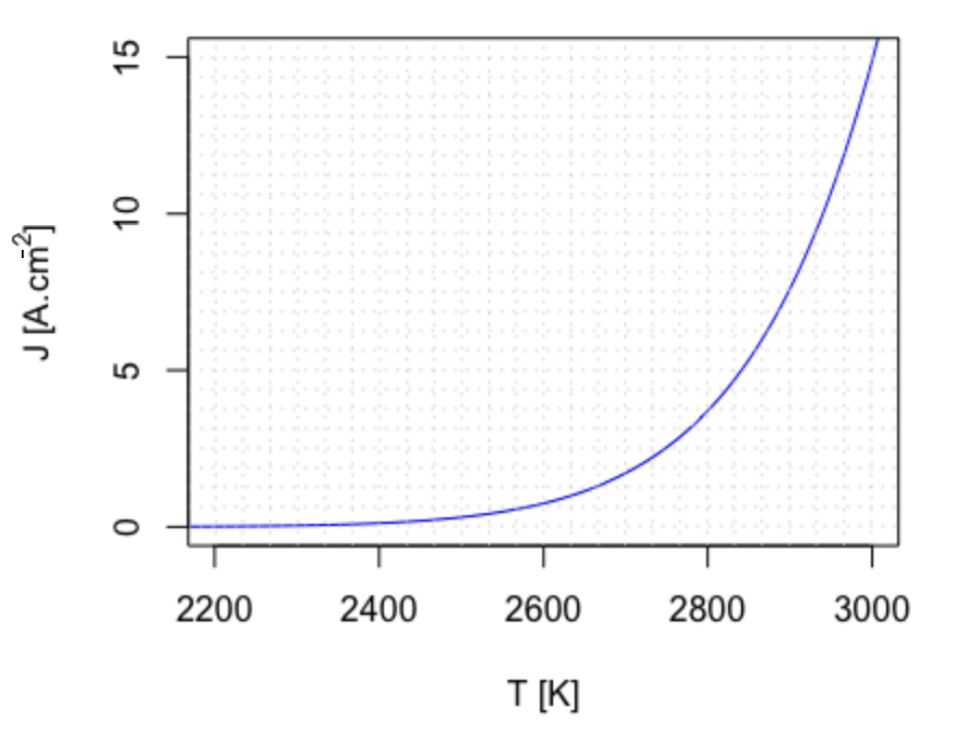
\includegraphics[width = 350 pt]{WolframGraf.png}
	\caption{Závislost emisního proudu $J$ z wolframu na jeho teplotě $T$ dle Richardson-Duschmanova vztahu (\ref{RDlaw}), pro wolfram $W=4,54$ eV a $B=60$ Acm\textsuperscript{-2}K\textsuperscript{2} ~\cite{zdrojwolf}.}
	\label{WolframGraf}
\end{figure}
\par Kvůli tepelné odolnosti a malé výstupní práci $W=4,54$ eV ~\cite{zdrojwolf} se jako emisního materiálu využívá zejména wolframu s možnými přiměsmi pro snížení výstupní práce. Navíc wolfram jako vodič může být zahříván pomocí ohmického ohřevu a být stálý i při teplotách okolo 3000 K. Jak lze vidět na Obr. \ref{WolframGraf}, kde je vyobrazen Richardson-Duschmanův vztah pro wolfram s $B=60$ Acm\textsuperscript{-2}K\textsuperscript{2} ~\cite{zdrojwolf}, při teplotách nad 2600 K z wolframu vyletuje vysoký proud elektronů. 
\par Musíme však vzít v potaz povrch námi použitého wolframového vlákna. Využili jsme wolframového vlákna stočeného do šroubovice se zruba $n=70$ závity, výška šroubovice je $h_s=0,5$ cm, průměr samotného vlákna byl $r=h_s/100$ cm a průměr podstavy opisovaného válce šroubovicí zhruba $d=6r$ ($h_s$ odpovídá výšce celého válce). Odsud lze vypočíst výšku válce potřebnou pro jednu otočku (\textit{revolution}) šroubovice jako $h_{rev}=h_s/n$, poté platí úvaha dle Obr. \ref{HevixUnWrap}, že rozvineme-li plášť tohoto malého válce s jednou otočkou šroubovice, tak dostaneme obdélník, jehož úhlopříčka je délka šroubovice na jednu otočku $l_{rev}$ a strany obdélníku jsou rovny $h_{rev}$ a $\pi d$, proto 
\begin{equation}
l_{rev}=\sqrt{h_{rev}^2+(\pi d)^2},
\end{equation}
odsud $l_{rev}\simeq 0,09$ cm. Jelikož otoček jsme měli právě $n=70$ a délka drátu na jednu otočku je $l_{rev}$, je celková délka rozbaleného drátu $l=nl_{rev}\simeq 6,6$ cm. Nyní lze již snadno vypočíst povrch šroubovice jako $S=2\pi r l$ s výsledkem $S=0,2$ cm\textsuperscript{2}. Odsud předpokládáme-li teplotu wolframového vlákna okolo 2600 K, což odpovída emitujícímu proudou okolo $0,625$ Acm\textsuperscript{-2}, tak z našeho vlákna emituje proud o hodnotě zhruba $J=0,129$ A, odpovídající $1,4\times 10^{17}$ elektronům za sekundu.
\begin{figure}[htbp!]
	\centering
	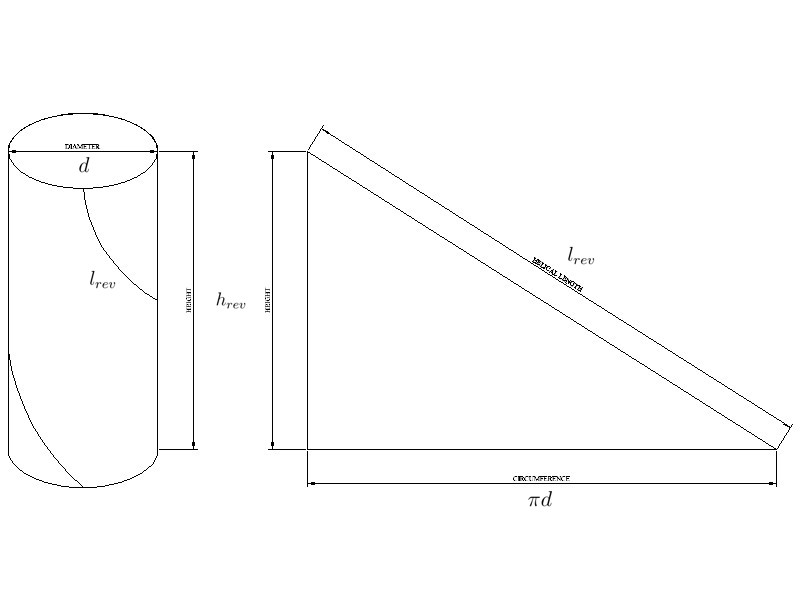
\includegraphics[width = 350 pt]{HevixUnWrap.jpg}
	\caption{Ilustrace odvození délky jednoho závitu šroubovice. Převzato a upraveno z~\cite{curv}.}
	\label{HevixUnWrap}
\end{figure}
\par Zvolili jsme ohmického ohřevu vlákna, kdy jsme připojili zdroj stejnosměrného napětí v rozmezí 0-15 V na svorky wolframového vlákna a do prostoru v okolí emitujícího vlákna umístili válcové anody pro urychlení elektronů a formování svazku, tento urychlovací a fokusační systém bude představen dále a v kapitole \ref{kapFok} a \ref{kapKuba}. V závislosti na napětí se měnilo i spektrum záření z wolframového vlákna, odkud jsme vizuálně odhadli dle modelu záření absolutně černého tělesa, že teplota vlákna přesahuje 2500 K při napětí nad 10 V. 
\par Jinou možností realizace termoemise je umístění ohřevného systému, např. i ohmického drátu, v okolí wolframové plošky či šroubovice, na které je přivedeno záporné napětí, tedy wolframová část je katodou. Kvůli ohřevnému systému dochází k termoemisi na wolframu, která je navíc stimulována napěťovým spádem mezi emitujícím wolframem a okolním prostorem. Tento druh termoemise je zajisté při stejných teplotách efektivnější, než termoemise indukovaná ohmickým ohřevem, protože zde navíc využíváme efektů podobných studené emisi, a to externího potenciálu.
\section{Urychlovací a fokusovací soustava elektrod}
Nyní bylo našim úkolem vytvořit soustavu elektrod sloužící ke správnému formování a urychlení svazku elektronů ze zdroje volných elektronů představených výše. Využívá se katody -- \textit{Wehneltova válce} obepínající zdroj elektronů k cílené prostorové emisi ve směru osy chtěného svazku. Aplikaci Wehneltova válce můžeme vidět na Obr. \ref{CFE}, kde je znázorněn jako část černého válce. Pro správnou volbu jeho geometrie spolu se sérií dalších urychlovacích a fokusovacích elektrod jsme v našem případě zvolili software SIMION (viz kap. \ref{kapKuba}) simulující chování elektronů ve vakuu v přítomnosti rotačně symetrických elektrod. Program dovoluje pro různé zdroje, tím s rozdílně energetickými i prostorově rozloženými elektrony, sestavit z dostupných elektrod teoreticky fungující model elektronového děla o daných vlastnostech svazku.
\par Nebudeme zde představovat první testované elektronové dělo z CRT monitoru, které jsme instalovali do vakuové komory a neúspěšně testovali. Bylo nutné určit napětí, které jsme přiváděli na jednotlivé elektrody, tento postup lze vidět v pololetní zprávě z tohoto projektového praktika -- PPRAK 2018/2019. Neúspěšnost při generaci elektronového svazku byla nejspíše zapříčiněna termoemisiním zdrojem elektronů, kdy bylo wolframové vlákno nejspíše přepálené.
\section{Vlastní elektronové dělo}
Rozhodli jsme se sestavit vlastní elektronové dělo využívající termoemise z wolframového vlákna (halogenová žárovka) a sérii válečkových měděných elektrod, jejichž vliv na formování svazku byl simulován pomocí programu SIMION. Sestavili jsme dvě aparatury využívající termoemise, avšak ani v jednom případě jsme na stínítku s fluorescenční vrstvou neviděli zelené světlo původem z interakce elektronů a atomů fluorescenční látky. Avšak při výbojích na některých z elektrod jsme na stínítku pozorovali záblesky zeleného světla, tím se domníváme, že urychlovací soustava byla funkční a problém byl ve zvoleném zdroji elektronů -- termoemisním wolframu. Z tohoto důvodu jsme vytvořili třetí setup, sestávající se z průmyslového děla, který jsme využili jako zdroj elektronů v rozmezí 0-5 keV spolu se soustavou elektrod mající za cíl kolimace a urychlení svazku elektronů až na energie okolo 20 keV. Vyšších energií elektronů jsme nemohli dosáhnout, neboť maximální napětí, které jsme byli bez probíjení schopni dovést do vakuové komory bylo právě 20 kV. Naším původním cílem bylo získat svazek elektronů o energiích až 80 keV.
\par V programu SketchUp jsme navrhli držáky a kolejnicovou platformu pro pozdější uchycení měděných válečků o průměru 3 cm. Finální verzi vytisknutá na 3D tiskárně PRUSA i3 MK2 pomocí materiálu APL lze vidět na Obr. \ref{SetUp} i v zapojení s elektrodami. Materiál APL vydrží vakuum až 10\textsuperscript{-7} Pa, proto jsme ho využili jako uchycení měděných válečků -- elektrod. Měděné válečky měly různé výšky a dle návrhu z programu SIMION byly rozestaveny tak, aby vzhledem k dostupným zdrojů stejnosměrného napětí bylo možné vytvořit optimální potenciálový spád pro produkci elektronového paprsku. Díky kolejnicového systému upevnění držáků jsme měli zaručenou souosost válečkových elektrod.
\begin{figure}[htbp!]
	\centering
	\includegraphics[width = 350 pt]{SetUp.png}
	\caption{První sestava elektronového děla s držáky z materiálu APL a čtyřmi měděnými elektrodami. Zleva halogenová žárovka a poté následující soustava elektrod.}
	\label{SetUp}
\end{figure}
\subsection{Soustava čtyř elektrod s termoemisí}
První setup z APL držáků a měděných válečků je na Obr. \ref{SetUp}, jak můžeme vidět, žárovka je vně první elektrody. První elektroda tedy není Wehneltovým válcem. Simulaci funkčnosti takové sestavy je možné vidět na Obr. \ref{05simulaceVlastniDelo}, u kterého se nachází i jednotlivá napětí přivedená na elektrody. Toto dělo při zapojení napětí i žhavení wolframového vlákna nejevilo známky produkce elektronového svazku, jelikož jsme nepozorovali excitaci fluorescenčního stínítka. Z toho důvodu jsme přešli k sestavě s vnořením wolframového vlákna do první elektrody, simulace je na Obr. \ref{05simulaceVlastniDeloWehnelt}, první elektroda neplní funkci Wehneltova válce, ale anody. Při tomto setupu jsme na poslední hlavní urychlovací elektrodu připojili kladné napětí 18 kV, jež bylo reálně možné přivést do vakuové komory bez probíjení v okolí propustek. 
\par Při obou nastaveních jsme však nepozorovali interakci elektronového svazku s fluorescenčním stínítkem. Funkčnost fluorescenčního stínítka jsme později ověřili, stejně tak tomu nasvědčovaly zelené záblesky při výbojích v komoře v době zapojení urychlovacích elektrod. Jelikož v tomto případě elektrony doletěly až na stínítko vzdálené od výboje více jak 20 cm, poukazuje to navíc i na funkčnost urychlovacích elektrod. Tedy problém byl nejspíše ve zdroji volných elektronů, tj. v termoemisi z ohmicky ohřívaného wolframového vlákna.
\subsection{Průmyslové elektronové dělo se soustavou elektrod}
Kvůli nefunkčnosti předešlých setupů elektronových děl jsme přistoupili k variantě zprovoznění průmyslového elektronového děla, které jsme využili jako zdroj elektronů, a kdy jsme následně vytvořili přídavnou urychlovací a fokusovací soustavu pro dosažení vyšších energií svazku. Průmyslové elektronové dělo dosahuje energií svazku maximálně 5 keV (kap. \ref{kapTomasT}), což by i pro konverzi elektronů na fotony skrze zlato-měděnou fólii nemuselo být dostatečné. Způsob detekce elektronů pomocí chipu X-CHIP03 a použitá metodika je v kap. \ref{kapMatej} a \ref{kapAnezka}. 
\par Simulace námi použité sestavy pro finální měření na chipu X-CHIP03 je v podkap. \ref{simulaceKuba} spolu s použitými nastaveními napětí na elektrodách. Nejdříve jsme ověřili funkčnost průmyslového elektronového děla pomocí fluorescenčního stínítka a pozorovali vliv na fokusaci svazku na stínítku změnami napětí v soustavě přidaných elektrod.
